\section{Introduction}
\label{intro}

% very general intro on ML
Machine Learning (ML) gained a huge success in the last decades, becoming one of the most popular and studied branches of artificial intelligence \cite{jordan2015machine}. ML methods are widely used in many fields of research, with the aim of obtaining a general working learning rule from input data, namely a prediction function, to be used for future predictions of never-seen-before data.
Specifically, ML algorithms have been widely exploited in industrial processes, playing a relevant role in a wide range of applications: Industry 4.0 \cite{angelopoulos2019tacklin}, healthcare \cite{kourou2015machine}, transportation \cite{hamner2010predicting}, natural science \cite{yao2008quantitative}, social media \cite{balaji2021machine}, fraud detection \cite{awoyemi2017credit} and so on.

% General intro on AD
Anomaly detection represents an important and widely used ML task, broadly applied in various domains and applications where the issue of monitoring unexpected data behaviour is essential. This task defines the process of identifying anomalous data, i.e., data being characterised by a different behaviour with respect to other data distinguishing itself from the rest of the dataset. To date, there is no unanimously accepted definition but broadly speaking, an anomalous point, often named equivalently anomaly or outlier, is defined \textit{as an observation that deviates so much from other observations as to arouse suspicion that it was generated by a different mechanism} \cite{hawkins1980identification}. Anomaly detection is commonly tackled in many industrial scenarios, such as credit card fraud detection \cite{ghosh1994credit}, insurance fraud detection \cite{fawcett1999activity}, insider trading detection \cite{donoho2004early}, medical anomaly detection \cite{wong2003bayesian}. In these dynamic and often complex contexts, the problem of detecting anomalies is crucial in order to predict and avoid failures as well as to perform fault detection. In many industrial processes in fact, data-driven approaches for smart monitoring (for example predictive maintenance) have a key role, allowing to identify and isolate faults and to prevent future sudden failures. To solve this problem, anomaly detection represents an efficient solution.
Generally, in this scenario a great amount of collected data are available but, since labelling is an expensive and time consuming process, there is a lack of ground truth labels, undoubtedly stating whether or not a point is anomalous. The learning problem therefore is unsupervised and the algorithm can just blindly look at the structure of the dataset, without a clear definition of what is an anomaly from the user perspective. Therefore unsupervised algorithms can only detect samples that exhibit some general property different to the rest of the dataset, for example some approaches look for points far from the majority, or detect points living in low density areas.

% Anomalies are domain specific
Unfortunately, anomalies are strongly domain specific \cite{foorthuis2021nature}: as stated above, since no official definition is given, the concept of what an anomaly is entirely relies on the application in question. Specifically, it may happen that a set of data has different anomalies based on the given application domain and that the same data may be considered anomalous in one domain but normal in another \cite{sejr2021explainable}. For instance looking at data acquired by a measuring instrument, the manufacturer might define anomalies as events where the instrument has a faulty behaviour while the end-user might be more interested in events where the measured process behaves in a previously unseen way \cite{barbariol2020self}. As a direct consequence, training a domain specific anomaly detector would require a full set of labeled data to capture the user definition of anomaly. 

% full set of labels are too expensive
In real world applications, assigning labels to input data pose a considerable challenge to take into account \cite{zhu2009introduction}. In order to train reliable models, a large amount of labeled data is needed but, in practical scenarios, labeled examples are limited or often too expensive and time-consuming to collect, leading to a huge issue to face. Obtaining labels requires an often too expensive cost to take care of since the labeling procedure is usually carried on by a human domain expert who manually labels each point with a time-consuming and demanding routine. Moreover, by definition anomalous points are rare and difficult to spot, making the problem a difficult challenge to be solved. 
%as well as extremely unbalanced one. 
%\gas{Forse toglierei la roba dell'unbalanced qua o lo scriverei diversamente} 

% unsupervised AD is used in practice, but has no precise anomaly definition
Due to the difficulty of finding labeled points, in practical contexts anomaly detection is often treated as an unsupervised learning task. For the classical unsupervised anomaly detection problem, the purpose is to detect outliers with no use of labeled data based on the fact that normal data greatly outnumbers anomalous data, and anomalies are very different with respect to inliers. Unsupervised anomaly detection models are not tuned for the precise domain of application but are generally based on identifying rules based on specific data characteristics, such as density based algorithms, distance based methods etc. \cite{hochenbaum2017automatic, hill2010anomaly, knorr1998algorithms, breunig2000lof}. 
However recent literature \cite{das2016incorporating,sejr2021explainable} distinguishes the outliers to the anomalies: the first are the points highlighted by an unsupervised model, while the second are the ones the user actually sees as anomalous. As the unsupervised model is not directly tuned to the detection of the anomalies, the outliers might weakly correlate with them. 

% outliers do not coincide with anomalies
Therefore, running unsupervised anomaly detection algorithms may be risky and often misleading: as stated above anomalies are strongly domain dependent and as a direct consequence, an unsupervised detector might not identify anomalous data which should be considered as such, as well as could wrongly detect as anomalies points which are normal based on the context taken under consideration \cite{das2016incorporating}. Figure \ref{anomalyvsoutlier} presents a visual representation of the strong connection between anomalous data points and context domain. Specifically, the plot shows the two-dimensional projection of the \textit{vowels} dataset \cite{Rayana}. As it can be seen, anomalies are not defined just as data points lying far or in low-density regions, but they form a class with a specific pattern defined by domain-experts, making complicated for the automatic detector to correctly identify them.

\begin{figure}
    \centering
    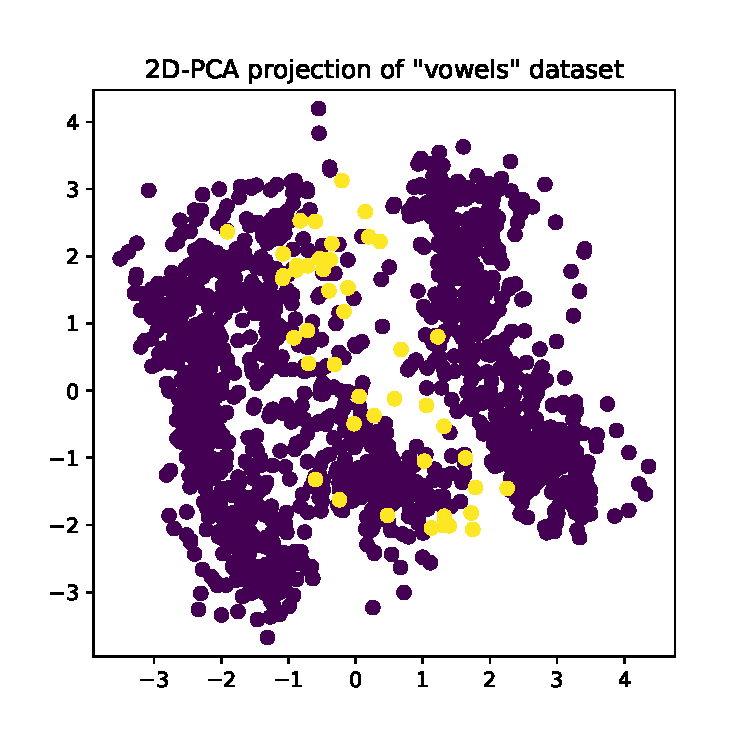
\includegraphics[scale=0.6]{vowelsPCA.pdf}
    \caption{Projection of the \emph{vowels} dataset on 2 dimensions using Principal Component Analysis. Purple data points are normal data, yellow points are anomalous data. Two aspects are clearly visible: i) it is impossible to separate anomalies from normal data with only two features and ii) anomalies tend to form a different class and might be quite different from general outliers. Not all the data points lying in low density areas or far from the majority are defined as anomalies, but just the ones lying in a specific part of the space. 
    %As shown, anomalies do not tend to have any peculiar discrepancies with respect to normal points. On the contrary, they lie on the same portion of space occupied by normal points.
   As a consequence, in the considered scenario, identifying anomalies might be a challenging task for an unsupervised detector.}
    \label{anomalyvsoutlier}
\end{figure}


% presentazione di IF
Among the unsupervised models, a very popular anomaly detection algorithm is the Isolation Forest (IF) \cite{liu2008isolation, liu2012isolation}, which presents a very different approach w.r.t. the majority of models: instead of creating a profile for normal data, it explicitly tries to isolate anomalies. To do it, IF relies on two assumptions: anomalies are fewer in number and they have very different attributes compared to normal data. 


%\gas{Manca imho il discorso: AD pervasiva -> ci sono i sistemi di supporto alle decisioni -> abbiamo ora la possibilità in tante applicazioni di ottenere una taggatura non costosa dopo aver sviluppato un primo sistema di Anomaly Detection}

In Decision Support Systems (DSS) \cite{keen1980decision}, data streams are analysed in order to quickly extract strategic decisions on complex problems. Such process is monitored by users who frequently interact with the system and represent the actual decision maker of the whole process. In such framework, \approach represents an extremely appealing approach. Specifically, if a DSS is present, as a direct consequence, a user is already overseeing the process and inspecting data points: considering an unsupervised anomaly detection problem, inexpensive labels may be obtained in a fast way and using \approach the model may be inexpensively updated. 


% novelty
In this paper we describe a procedure able to tune the detector model on domain specific anomalies by interacting with a human expert. To perform the proposed tuning method, not every training data are presented and labeled but a subset is automatically selected so that the number of interactions between the system and the human is minimised. The core idea is to ask labels corresponding to the most significant points to reduce the labeling cost and at the same time to maximize the detection performance. As a direct consequence, the proposed procedure may be regarded as an Active Learning (AL) based model \cite{kumar2020active}. 

\begin{figure}
\centering
\usetikzlibrary{automata, arrows.meta, positioning}
 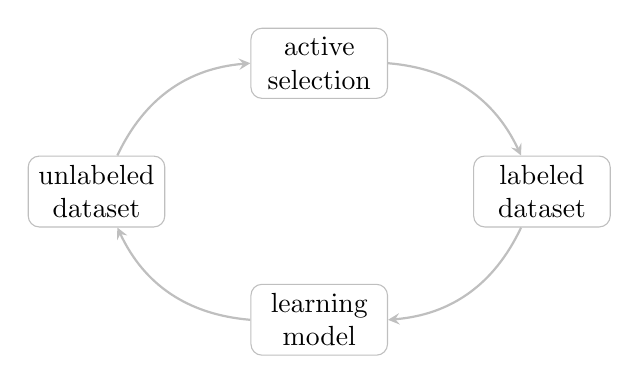
\begin{tikzpicture} [node distance = 4cm, on grid, auto]
 
\node (q0) [draw,lightgray, rounded corners, text width=1.5cm,yshift=-1.2cm, align =center] {\textcolor{black}{unlabeled \\dataset}};
\node (q1) [draw,lightgray, text width=1.5cm, rounded corners,above right = of q0,  yshift=-1.2cm,align =center] {\textcolor{black}{active \\selection}};
\node (q2) [draw,lightgray,rounded corners, text width=1.5cm, below right = of q1,yshift=1.2cm,align =center] {\textcolor{black}{labeled \\dataset}};
\node (q3) [draw,lightgray,rounded corners, text width=1.5cm, below left = of q2,yshift=1.2cm,align =center] {\textcolor{black}{learning \\model}};
 
\path [-stealth, thick]
    (q0) edge [lightgray, bend left]  (q1)
    (q1) edge [lightgray,bend left]  (q2)
    (q3) edge [lightgray,bend left]  (q0)
    (q2) edge [lightgray,bend left]  (q3);
\end{tikzpicture}
\caption{Active learning core structure. At each iteration a novel point is actively selected from the unlabeled set of data and the corresponding label is requested. Based on the received information, the model is modified.} \label{al}
\end{figure}

Indeed AL represents a training approach particularly suitable when labeled samples are too expensive or difficult to obtain. Specifically, AL is a particular ML algorithm based on a key idea: despite the shortage of labeled data, high accuracy results may be obtained if the training algorithm is allowed to choose the points to be labeled and learn from them \cite{settles1995active}. An AL algorithm asks an oracle to label the data considered most informative with an iterative approach. Doing so, since the queried points are directly selected by the learning algorithm, the amount of necessary labeled data is much smaller than that required for classical supervised ML approach. Figure \ref{al} shows the core structure of any AL algorithm: at each iteration the model is updated using the labelled dataset, and is allowed to ask for a new label in the unlabelled dataset. This process repeats until the model reaches sufficient performances or when the number of iterations reaches the maximum budget.

%\\In recent years, some active learning-based anomaly detection algorithms have been proposed.
%The idea of incorporating expert feedback in unsupervised anomaly detection algorithms aims at improving the achieved performance adding a relatively small computational cost. Active anomaly detection (AAD) algorithm \cite{das2016incorporating, das2017incorporating} proposes an active learning anomaly detection approach where points are ranked based on their anomalous behavior. The main goal is to maximize the number of true anomalies presented to the domain expert. An inclusion of AAD algorithm in the One Class Support Vector Machine (OCSVM) framework is tackled in \cite{lesouple2021incorporating}.
%Always using OCSVM, an expert feedback inclusion has been recently proposed %\cite{lesouple2021introduce}: to solve the problem, the paper combines together the $\mu$-SVM for the %labeled data and the OCSVM for the unlabeled set of data.

This paper focuses on the Isolation Forest detector, and suggests a strategy to tune it towards the user definition of anomaly. In this work the authors compare two AL query policies to ask the user new labels, and other two policies to update the internal structure with minimal computational effort. The goal is to increase the performance of the detector as much as possible, keeping very low both the labelling effort and the updating procedure. Moreover this method has two key advantages over the supervised and computationally expensive models: as it relies on an initial unsupervised training, it can start to work when there are no labels, but more importantly it can work even if instances from only one class are labelled. This is particularly useful when obtaining labels from the anomalous class is very uncommon or expensive.

%\gas{The rest of the papers is organized as follows: ...}
The rest of the paper is organized as follows. Initially, in Section \ref{rw} we outline the Isolation Forest in detail, and we indicate an existing active learning-based anomaly detection algorithm that will be used as a benchmark in thos work. Then, in Section \ref{pm} we illustrate the proposed model \approach: namely, we describe the strategies suggested to query the points as well as the approaches employed to update the model. In Section \ref{exp} we test \approach, comparing it with other models in relation to multiple real set of data. Finally, in Section \ref{conclusions} we draw conclusions for the present work.

%This paper compares two AL query strategies for anomaly detection using Isolation Forest. The algorithm key idea is to modify the internal structure of the unsupervised model based on a small amount of labeled data queried to the domain expert, trying to minimize the labelling effort but at the same time maximising the detection performance. Specifically, the presented model is based on the Isolation Forest model, i.e., the basic concept used to classify anomalies remains isolating data points from the rest of the dataset. Anyway, an innovative approach is used to query the labels and to update the model: novel information is achieved with the use of an active learning strategy by which the inner framework of the model is modified in order to match with the information obtained. Once the information is achieved, a user friendly iterative process allows to adapt the model by adjusting its structure on the basis of the novel input.
%The proposed method relies onto two distinguished yet essential issues: a process to select the most significant points and a tuning procedure to modify the structure of the model based on the information achieved. 
%This method has two key advantages over the supervised computationally expensive models: it is extremely computationally efficient and works even if instances from only one class are labelled.
%Based on the treated framework and on the data in hand, active learning algorithms are characterized by many possible query strategies \cite{settles1995active}. In this way, based on the considered purpose, the suitable query strategy may be selected and the corresponding most informative point may be labeled. 
%In the same way, we propose two possible approaches to address the selection of points to be labeled, producing two different query strategies with respect to both their benefits as well as their computational costs.
%\tommi{bisognerebbe scrivere che testiamo il nostro metodo su dataset reali e pubblichiamo il codice bla bla bla.}
%The importance of the algorithm...
%As we will see later the proposed model is based on...
%Section \ref{} ecc..
%list of the notation - simboli usati fare tabella





%\tommi{monitoring unexpected behaviour?} is essential. 
 %Even if, to date, there is no clear or official definition, broadly speaking, an anomalous point, also known as anomaly or outlier, is defined \textit{as an observation that deviates so much from other observations as to arouse suspicion that it was generated by a different mechanism} \cite{hawkins1980identification}. In general, an anomaly is identified as a variation from the norm, a data being characterised by a different behaviour with respect to other data that distinguishes itself from the rest of the dataset. Consequently, anomaly detection algorithms aim at detecting or identifying data that seem not to conduct themselves with a standard trend.
%\tommi{non sembra che parliamo di distribuzione gaussiana?}. 
%Anomaly detection techniques may be divided into three groups based on the available data in use: supervised, unsupervised and semi-supervised. 
%If the dataset contains labeled data, any technique for binary classification may be used, leading to highly accurate results. 
%Unfortunately, a critical challenge of anomaly detection is the lack of labeled data \cite{chandola2009anomaly}. Obtaining labels requires an often too expensive cost to take care of, since the labeling procedure is usually carried on by a human expert domain who, by hand labels each point with a time consuming and demanding routine. To solve this matter, semi-supervised or unsupervised techniques are employed. In the first scenario, a labeled portion of the original dataset is required, usually belonging to the most representative normal class, and, based on such labeled data, a model representing the normal behaviour is produced. \tommi{dici?} Generally, in fact, labeling normal data requires less efforts: normal points tend to have a common and more static behavior, making it easier to  be identified.
%For the classical unsupervised anomaly detection problem, the purpose is to isolate outliers with no use of labeled data based on the fact that normal data greatly outnumbers anomalous data. As a rule, unsupervised anomaly detection models are not tuned for the precise domain of application but are generally based on identifying rules based on specific data characteristics. 
%Based on the context and on the problem in question, different popular anomaly detection techniques exist. 
%\tommi{tornarci} A large class of unsupervised anomaly detectors are those based on statistical methods. These techniques produce a statistical distribution based on the given set of data and classify points according to where data falls: points that are not consistent or that simply lie in the tails of the computed distribution are consider anomalies \cite{hochenbaum2017automatic, hill2010anomaly}. 
%Some anomaly detection methods are based on the traditional classification problem. Based on the classical Support Vector Machine framework several methods have been proposed: the one-class support vector machine \cite{scholkopf1999support} computes an hyperplane that separates the data points from the origin and at the same time maximizes its distance with respect to the origin; the support vector data description \cite{tax2004support} looks for the smallest hypersphere containing the considered dataset. Distance-based \cite{knorr1998algorithms} and density-based \cite{breunig2000lof} outlier detection methods try to solve the problem by finding a profile for normal data based on inner data characteristics: the first uses the average distance of points, since, by nature, outliers have a higher value with respect to normal points; the latter is based on density area, due to the fact that outliers tend to stay in low density areas compared to normal points, which usually assemble in the same area. 

% tommi: andrei a capo in modo da evidenziare IF che è il metodo che andremmo ad analizzare
%A very popular anomaly detection algorithm is the Isolation Forest algorithm \cite{liu2008isolation, liu2012isolation}, which presents a brand-new approach: instead of creating a profile for normal data, it explicitly tries to isolate anomalies. To do it, Isolation Forest relies on two anomaly inner characteristics: they are fewer in number and they have very different attributes compared to normal data. 

%To cope with the lack of labeled data, in recent years some active learning-based anomaly detection algorithms have been proposed.
%The idea of incorporating expert feedback in unsupervised anomaly detection algorithms aims at improving the achieved performance adding a relatively small computational cost. Active anomaly detection (AAD) algorithm \cite{das2016incorporating, das2017incorporating} propose an active learning anomaly detection approach where points are ranked based on their anomalous behavior. The main goal is to maximize the number of true anomalies presented to the domain expert. An inclusion of AAD algorithm in the One Class Support Vector Machine (OCSVM) framework is tackled in \cite{lesouple2021incorporating}.
%Always using OCSVM, an expert feedback inclusion has been recently proposed \cite{lesouple2021introduce}. To solve the problem, the paper combines together the $\mu$-SVM for the labeled data and the OCSVM for the unlabeled set of data. 
%\cite{vercruyssen2018semi}. 


%This paper presents a novel active learning strategy for anomaly detection using Isolation Forest. The algorithm key idea is to modify the internal structure of the unsupervised model based on a small amount of labeled data queried to the domain expert, trying to minimize the labelling effort but maximising the detection performance. Specifically, the presented model is based on the Isolation Forest model, i.e., the basic concept used to classify anomalies remains isolating data points from the rest of the dataset. Anyway, an innovative approach is used to query the labels and to update the model: novel information is achieved with the use of an active learning strategy by which the inner framework of the model is modified in order to match with the information obtained. Once the information is achieved, a user friendly iterative process allows to adapt the model by adjusting its structure on the basis of the novel input.
%Based on the treated framework and on the data in hand, active learning algorithms are characterized by many possible query strategies \cite{settles1995active}. In this way, based on the considered purpose, the suitable query strategy may be selected and the corresponding most informative point may be labeled. 
%In the same way, we propose two possible approaches to address the selection of points to be labeled, producing two different query strategies with respect to both their benefits as well as their computational costs.
%\tommi{bisognerebbe scrivere che testiamo il nostro metodo su dataset reali e pubblichiamo il codice bla bla bla.}
%The importance of the algorithm...
%As we will see later the proposed model is based on...
%Section \ref{} ecc..
%list of the notation - simboli usati fare tabella

\begin{comment}
\begin{table*}[]
    \centering
    \begin{tabular}{ll}
    \hline
          \textbf{Symbol} & \textbf{Description} \\
         \hline
         $X$ & generic sample set \\
          $X'$ & generic sub sample set \\
         $\psi$ & sub-sample set size\\
          $s(x,\psi)$ & anomaly score of generic point $x$\\
         $E(h(x))$ & average path length of generic point $x$\\
          $c(\psi)$ & average path length of an unsuccessful search \\
          & in a binary search tree \\
         
         $\mathcal{U}=\{x^i,\dots,x^n\}$ & unlabeled sample dataset \\ & ($x^i \in \mathbb{R}^m$) \\
          $n$ & number of observations \\
          $T_p$ & generic iTree \\
           $l$& generic leaf\\
          $l_a$ & numbered of labeled anomalous points in $l$\\
           $l_n$ & numbered of labeled normal points in $l$\\
          $k$ & \textit{color} of $l$\\
           $p(l)$& leaf coefficient of $l$\\
          $h(p)$ & synthetic depth of $l$\\
           $h_{max}$ & maximum depth of an iTree\\
          $h_{min}$ & minimum depth of an iTree \\
          $\tau$ & threshold value\\
          $t$ & number of iTrees\\
          $\hat{x}$ & selected queried point \\
           $\hat{y}$ & requested true label \\
         \hline
    \end{tabular}
    \caption{List of symbols used. }
    \label{list_sym}
\end{table*}
\end{comment}


\begin{table*}[]
    \centering
    \begin{tabular}{ll}
    \hline
         \textbf{Symbol} & \textbf{Description} \\
         \hline
         $X$ & generic sample set \\
         $X'$ & generic sub-sample set ($|X'|= \psi$) \\
         $X^\mathcal{s}$ & set of labelled training points\\
         $X^\mathcal{u}$ & set of unlabelled training points \\
         $n_x$ & number of observations in $X$\\
         $n_\mathcal{s}$ & number of observations in $X^\mathcal{s}$\\
         $n_\mathcal{u}$ & number of observations in $X^\mathcal{u}$\\
         $x_j$ & $j-$th queried point\\
         %$\cdot_j$ & $j-$th queried point\\
         $F$ & forest \\
         $T$ & tree \\
         $n_T$ & number of trees\\
         $L$ & leaf \\
         $n_L$ & number of leaves \\
         $L_\mathcal{p}$ & partition of $X$ made by $L$\\
         $L_\mathcal{h}$ & depth of $L$\\
         $L_\mathcal{i}$ &  number of normal points in $L$\\
         $L_\mathcal{o}$ & amount of anomalies contained in $L$ \\
         $a(x)$ & anomaly score of generic point $x$ \\
         $h^\mathcal{u}(x)$ & "unsupervised" path length of generic point $x$ \\ 
         $h^\mathcal{s}(x)$ & "supervised" path length of generic point $x$ \\ 
         $k(L)$ & color of leaf $L$\\
         $\lambda_T(x)$ & compute leaf containing $x$ with respect to tree $T$\\
         $H_{jt}$ & compute the path length of $x_j$ with respect to tree $T_t$\\
         $H \in \mathbb{R}^{n_T \times n_\mathcal{u}}$ & matrix of elements $H_{jt}$ \\
         \hline
    \end{tabular}
    \caption{List of symbols used.}
    \label{list_sym}
\end{table*}